\documentclass{article}

\usepackage{neurips_2026}

\usepackage[utf8]{inputenc}
\usepackage[T1]{fontenc}
\usepackage{hyperref}
\usepackage{url}
\usepackage{booktabs}
\usepackage{amsfonts}
\usepackage{amssymb}
\usepackage{amsmath}
\usepackage{nicefrac}
\usepackage{microtype}
\usepackage{xcolor}
\usepackage{graphicx}
\usepackage{array}
\usepackage{enumitem}
\usepackage{placeins}

\newcommand{\method}[1]{\texttt{#1}}
\newcommand{\wstar}{W^{\star}}
\newcommand{\mstar}{M^{\star}}
\newcommand{\cstar}{C^{\star}}

% TODO(camera-ready): venue retarget — this skeleton uses the NeurIPS 2026
% style shared by the companion papers; retarget to ICLR 2027 / AAMAS 2027
% class before submission.

\title{Semantic Warp: Provenance-Conditioned Completion\\in Collective Memory}

%\author{%
%  Anonymous Authors \\
%  Anonymous Institution \\
%  \texttt{anonymous@anonymous.edu} \\
%}

\begin{document}

\maketitle

\begin{abstract}
\textbf{Problem.} In collective memory for multi-agent navigation, an agent can commit to --- and reach --- a target it has never observed: all supporting evidence arrived from peers. Folk culture calls this navigating by someone else's song; we call it a \emph{semantic warp}. Success-only and even stage-level metrics cannot see it, because no existing evaluation conditions completion on the \emph{provenance} of the evidence behind the commitment.
\textbf{Approach.} We define the warp event $\wstar_\theta := \mstar \wedge (\varphi \ge \theta)$, where foreignness $\varphi$ is the peer share of the evidence mass \emph{in the same weights the merge used to select the candidate}, frozen at lock time. Warp is not a fifth Q/R/M/C stage but an annotation that splits $P(\cstar|\mstar)$ into provenance strata. Because symbolic merges decompose by source, we obtain (i) a counterfactual attribution of warp value via deterministic replay with foreign evidence masked, (ii) a closed-form \emph{warp distance law} from trust$\times$staleness rules, and (iii) a decentralised \emph{Warp Drive} protocol (optimistic lock + reservation + anti-$\mstar$ rollback) for the warp-collision pathology.
\textbf{Findings.} On a 2{,}400-episode scarcity sweep, raw warp locks almost never complete directly ($P(\cstar|\wstar)=0.004$--$0.020$ vs.\ $0.22$--$0.41$ for own locks; CIs disjoint), yet foreign evidence still carries value as transport: up to $51\%$ of own-lock completions are warp-assisted chains. The distance law predicts intention-formation horizons tick-exactly, including a $6/6$-exact hold-out with predictions registered before execution. Warp Drive turns the trade-off around: success rate rises at every cadence (disjoint CIs), and fast sharing with the protocol beats the best fixed-cadence baseline ($0.614$--$0.620$ vs.\ $0.583$). A cross-session, cross-agent strict warp is replicated on an LLM substrate ($10/10$ layouts vs.\ $0/10$ without foreign memory).
\textbf{Thesis.} The value of collective memory lies less in the information itself than in the \emph{coordination contract attached to the information}.
\textbf{Scope.} Grid-world substrates and one small text-world LLM demo; the contribution is a measurement layer, a falsifiable law, and a minimal protocol, not a general theory.
\end{abstract}

\section{Introduction}
\label{sec:intro}

In songline cultures, a traveller who knows the song can cross terrain
they have never seen: navigational competence transfers without
physical visitation. Multi-agent systems with shared memory perform
the same act constantly --- an agent commits to a water source, a goal
region, or a tool location known only from a peer's broadcast --- yet
no standard evaluation distinguishes this act from ordinary
memory-driven navigation. Success metrics aggregate over it;
stage-level diagnostics such as Q/R/M/C count the commitment
($\mstar$) and the completion ($\cstar$) but not \emph{whose evidence}
backed them.

This paper makes that act a first-class measured event. A
\emph{semantic warp} $\wstar$ is a target materialisation whose
supporting evidence mass is (almost) entirely foreign, and
\emph{warp completion} $P(\cstar|\wstar)$ asks whether someone else's
song actually gets you there. Three properties of symbolic collective
memory make the construction sharp, and none of them holds for opaque
vector memories:

\begin{enumerate}[leftmargin=20pt,itemsep=2pt,topsep=2pt]
\item \textbf{Merges decompose by source.} Foreignness
  $\varphi\in[0,1]$ is computed from the same per-source weights
  (trust, staleness, support) the merge itself used to rank the
  candidate --- it is a reading of the decision, not a new heuristic.
\item \textbf{Replays are deterministic.} Re-running an episode with
  foreign contributions masked at merge yields a \emph{counterfactual}
  warp gain per episode, not a correlation.
\item \textbf{Sharing rules have closed forms.} Trust and staleness
  decay imply a \emph{warp distance law}: an explicit horizon beyond
  which foreign evidence can no longer form intention --- falsifiable,
  and falsifiably different across architectures.
\end{enumerate}

Our measurements then force a reframing. Raw warp is nearly worthless
at the point of completion: under scarcity, warp locks complete an
order of magnitude less often than own-evidence locks
(\S\ref{sec:raw}), because concurrent recipients of the same broadcast
race for the same target and most must lose. Yet the same foreign
evidence is demonstrably valuable as \emph{transport}: up to half of
all own-evidence completions are chains that began with a failed warp
lock which carried the agent into self-confirmation range
(\S\ref{sec:taxi}). And a lightweight decentralised contract --- a
reservation piggybacked on the existing broadcast plus an
anti-$\mstar$ rollback in the sense of Time Warp
simulation~\cite{jefferson1985}
--- recovers what raw warp loses: with the protocol, \emph{fast}
sharing becomes the best-performing regime on unconditional success
rate (\S\ref{sec:drive}). Hence the thesis in one sentence:
\textbf{the value of collective memory is not the information; it is
the coordination contract attached to the information.}

\paragraph{Contributions.}
\begin{enumerate}[leftmargin=20pt,itemsep=2pt,topsep=2pt]
\item The first provenance-conditioned completion metric for
  collective memory: $\wstar_\theta$, $\varphi$ frozen at lock time,
  the decomposition
  $P(\cstar|\mstar)=P(\cstar|\mstar,\varphi{<}\theta)\,P(\varphi{<}\theta|\mstar)
  + P(\cstar|\wstar)\,P(\wstar|\mstar)$, and the counterfactual warp
  gain via source-masked deterministic replay
  (\S\ref{sec:warp-def}--\S\ref{sec:raw}).
\item The \emph{warp distance law}
  $\mathrm{age}_{\max}(\tau_i)=\alpha^{-1}\ln(\tau_i c/\tau)$ derived
  from the memory's own trust$\times$staleness rules, validated
  tick-exactly including a registered-prediction hold-out ($6/6$
  exact, one cell where a pruning horizon must undercut the
  exponential gate --- and does) and an architecture-level shape
  difference: fixed-cadence peer memory has \emph{no} gate
  (\S\ref{sec:law}).
\item The \emph{Warp Drive} protocol: optimistic warp lock,
  reservations carried on the existing broadcast cadence (no
  coordinator), and anti-$\mstar$ rollback with exponential backoff.
  It resolves the known misled-agent pathology preventively, bounds
  rollback latency by ${\approx}K$ ticks, and lifts unconditional
  success rate above the best fixed-cadence baseline
  (\S\ref{sec:drive}).
\item A cross-session, cross-agent strict warp on an LLM substrate:
  an agent that has never observed a room solves a task there purely
  on another agent's previous-session memory, replicated $10/10$
  layouts against a $0/10$ control (\S\ref{sec:llm}).
\end{enumerate}

\paragraph{Relation to the companion papers.}
The Q/R/M/C framework paper treats stage rates as the measurement
instrument; the collective-memory paper establishes the architectures
and the cadence trade-off. This paper adds the provenance axis on top
of both: the same logs, one new annotation, and the mechanisms the
annotation exposes. % TODO: cite companions per venue policy.

\section{Setting}
\label{sec:setting}

\paragraph{Substrate and task.} $N$ agents explore a $12\times10$ grid
with $M$ semantic water targets ($N>M$: scarcity) and hazards. Each
agent maintains symbolic place memory (tags, confidences, support,
freshness). Four sharing architectures over the identical substrate
and planner: \method{independent} (no communication),
\method{shared} (single event bus), \method{centralized} (consensus
aggregator), \method{peer} (broadcast every $K$ ticks, asymmetric
trust), plus \method{CSM} (peer $+$ explicit merge/trust/staleness
rules with decay rate $\alpha{=}0.05$ and inclusion threshold
$\tau{=}0.30$). % TODO: compress substrate details; cite companion §2.

\paragraph{Q/R/M/C instrumentation.} Per tick and per agent we log
query formation (Q), retrieval satisfaction (R), target
materialisation as the planner's lock ($\mstar$), and completion
($\cstar$). Episode-level conditional rates follow the companion
definition. All warp measurements below are annotations of these
$\mstar$ events; no planner or memory invariant is modified.

\section{The warp event}
\label{sec:warp-def}

\paragraph{Provenance and foreignness.} Every evidence unit entering a
merge carries its source. For the candidate $m$ the planner locks,
\[
\varphi(m) \;=\;
\frac{\sum_{e\in\mathrm{supp}(m),\,\pi(e)\neq\mathrm{self}} w(e)}
     {\sum_{e\in\mathrm{supp}(m)} w(e)},
\]
where $w(e)$ are \emph{the merge's own weights}: $\text{trust}\cdot
\log(1{+}\text{support})$ for peer/centralized consensus,
$\text{trust}\cdot e^{-\alpha\,\text{age}}\cdot\text{conf}$ for CSM,
observation masses for the shared bus. For peer and centralized
architectures $\varphi$ is reconstructed exactly from the
per-contribution fields the merge already exports; the measurement
layer reads state and never writes it.

\paragraph{Freezing rule.} $\varphi$ is fixed at the moment of the
lock. If the agent later confirms the place with its own eyes,
$\varphi$ is \emph{not} recomputed --- otherwise every successful warp
would dilute itself on approach and $P(\cstar|\wstar)$ would be
unmeasurable by construction.

\paragraph{Warp events and strata.} $\wstar_\theta := \mstar \wedge
(\varphi\ge\theta)$ with $\theta{=}1$ (strict: never self-observed,
cross-checked against an observation ledger) and $\theta{=}0.8$
(soft). Warp share $P(\wstar|\mstar)$ is a structural descriptor
(identically $0$ for \method{independent}); warp completion
$P(\cstar|\wstar)$ is the new quantity. The chain-rule decomposition
in \S\ref{sec:intro} makes warp an exact refinement of
$P(\cstar|\mstar)$, not a new stage: identifiability of Q/R/M/C is
untouched.

\paragraph{Regression anchor.} The known misled-agent episode of the
architecture comparison (agent A locks $(3,8)$ known only from C; C
claims it first; A strands) is annotated by the instrumentation as
$\varphi=1.0$ strict $\wstar$ with collision --- the pathology the
framework must see, and the protocol of \S\ref{sec:drive} must fix.

\section{Raw warp rarely completes --- but transports}
\label{sec:raw}

\paragraph{Design.} $2{,}400$ episodes: $(N,M)\in\{(3,2),(5,3),(8,5),
(4,4),(6,2)\}$ $\times$ three layouts $\times$
$\{\text{peer-}K2,\text{peer-}K8,\text{CSM-}K8,\text{shared}\}$
$\times$ 20 seeds $\times$ \{full, foreign-masked\} with identical
seeds. Unit of analysis: lock event; CIs by episode-cluster bootstrap.

\begin{figure}[t]
\centering
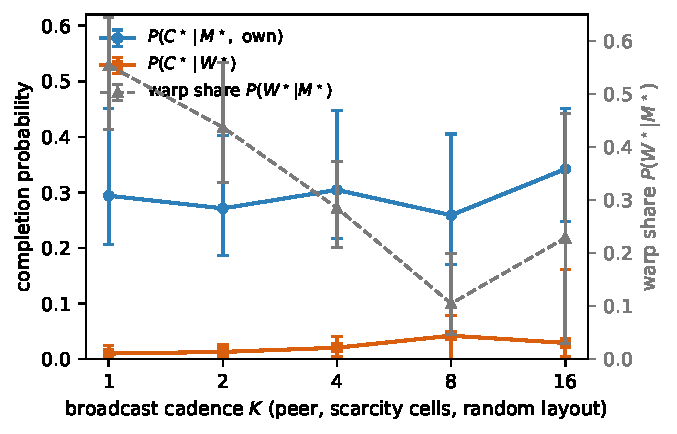
\includegraphics[width=0.72\linewidth]{figures/fig_warp_strata}
\caption{$\varphi$-stratified completion vs.\ broadcast cadence $K$
(dedicated peer sweep: scarcity cells, random layouts, 20 seeds,
episode-cluster bootstrap CIs). As $K$ shrinks, the warp share
$P(\wstar|\mstar)$ grows from $0.11$ to $0.55$ while
$P(\cstar|\wstar)$ stays below $0.05$ and the own-stratum rate stays
flat: the completion collapse of fast sharing is concentrated in the
$\wstar$ stratum, giving the companion paper's bottleneck shift its
mechanistic reading. The share uptick at $K{=}16$ (broadcasts are
rare, but agents also discover little on their own) is reported as
observed.}
\label{fig:strata}
\end{figure}

Figure~\ref{fig:strata} shows the cadence view on a dedicated peer
sweep ($K\in\{1,2,4,8,16\}$): warp share is what fast sharing buys,
and it is precisely the stratum that does not complete.
Table~\ref{tab:hw1} gives the architecture view.

\begin{table}[h]
\centering
\caption{Provenance strata of completion under scarcity ($N>M$), full
runs. Warp locks complete an order of magnitude less often than
own-evidence locks; all CI pairs are disjoint. (H-W1 confirmed.)}
\label{tab:hw1}
\small
\begin{tabular}{lcccc}
\toprule
Architecture & $P(\cstar|\wstar_{0.8})$ & $n_{\wstar}$ & $P(\cstar|\mstar,\text{own})$ & $n_{\text{own}}$ \\
\midrule
peer-$K{=}2$ & 0.004 [0.001, 0.008] & 1{,}437 & 0.223 [0.186, 0.275] & 2{,}738 \\
peer-$K{=}8$ & 0.020 [0.000, 0.038] & 149    & 0.389 [0.329, 0.446] & 1{,}734 \\
CSM-$K{=}8$  & 0.017 [0.006, 0.044] & 637    & 0.414 [0.368, 0.453] & 1{,}684 \\
shared       & 0.004 [0.002, 0.008] & 2{,}099 & 0.279 [0.237, 0.332] & 2{,}250 \\
\bottomrule
\end{tabular}
\end{table}

\subsection{Warp as transport: lock chains}
\label{sec:taxi}

Direct completion understates the value of foreign evidence. A
\emph{warp-assisted own completion} is a completed own-evidence lock
preceded (same agent, same episode) by a soft-$\wstar$ lock that was
dropped: the warp failed as a destination but succeeded as a ride.

\begin{table}[h]
\centering
\caption{Lock-chain analysis (random layouts, full runs). The first
$\wstar$ lock in a chain is made from ${\approx}8$--$10$ cells away;
the completing own lock from $2.0$ cells --- exactly the observation
radius, i.e.\ the self-confirmation point.}
\label{tab:taxi}
\small
\begin{tabular}{lccc}
\toprule
Arm & own $\cstar$ & warp-assisted (share) & $r(\text{first }\wstar) \to r(\text{own})$ \\
\midrule
shared          & 248 & 127 (\textbf{51.2\%}) & $9.5 \to 2.0$ \\
peer-$K{=}2$    & 223 & 99 (\textbf{44.4\%})  & $9.7 \to 2.0$ \\
CSM-$K{=}8$     & 279 & 13 (4.7\%)            & $5.8 \to 2.0$ \\
peer-$K{=}8$    & 246 & 7 (2.8\%)             & $8.4 \to 2.0$ \\
\bottomrule
\end{tabular}
\end{table}

This resolves an apparent paradox in the counterfactual data: the
shared bus at moderate scarcity gains $+10.8$ ticks $[+2.2,+20.9]$
from foreign evidence although its direct $P(\cstar|\wstar)$ is
$0.004$. The gain flows through chains; the freezing rule books the
completion honestly in the own stratum, and the chain analysis
recovers the warp's contribution as a separate measured quantity.

\subsection{Counterfactual warp gain}
\label{sec:gain}

Masking foreign evidence at merge under the same seed gives
$\mathrm{WG} = t_{\text{cens}}(\text{masked}) -
t_{\text{cens}}(\text{full})$ per episode. The sign map over (layout,
scarcity $\rho{=}N/M$) is regime-dependent: positive for the shared
bus at unpredictable layouts and moderate scarcity ($+10.8$ at
$\rho{=}1.5$), negative for fast peer sharing (peer-$K2$ random:
$-7.1$ $[-13.5,-1.3]$), ${\approx}0$ at hard scarcity. A per-agent
mask (one agent masked, others share normally) confirms the sign at
the individual level: $\mathrm{WG}_i = -10.25$ $[-20.91,-0.16]$ ticks
on the fast-share scarcity cell, with spillover on unmasked agents
${\approx}0$ ($-0.62$ $[-3.06,+1.91]$). Raw warp \emph{hurts} its
recipient precisely where sharing is fastest --- the collision cost
exceeds the information value. % TODO: full sign map to appendix.

\paragraph{Exploratory: collision pressure.} Co-lock pressure (other
agents locked on the same target) correlates with warp failure with
the predicted sign but negligible magnitude (Spearman $+0.033$,
$p{=}0.018$, $n{=}5{,}117$); we report it as exploratory rather than
as a confirmed predictor. % honest downgrade of pre-registered H-W5

\section{The warp distance law}
\label{sec:law}

CSM includes foreign evidence with weight $\tau_i\, e^{-\alpha\,
\text{age}}\, c$ (trust $\tau_i$, confidence $c{=}0.95$) and inclusion
threshold $\tau{=}0.30$. Foreign evidence therefore stops forming
intention at
\[
\mathrm{age}_{\max}(\tau_i) \;=\; \tfrac{1}{\alpha}\,
\ln\!\big(\tau_i\, c / \tau\big), \qquad \text{defined for } \tau_i c > \tau .
\]

\paragraph{Witness--traveller protocol.} A witness observes water once
and goes silent; a traveller who has never seen it receives the
snapshot at a parameterised age. Every lock the traveller makes is a
strict $\wstar$ by construction. Figure~\ref{fig:law} summarises both
experiments.

\begin{figure}[t]
\centering
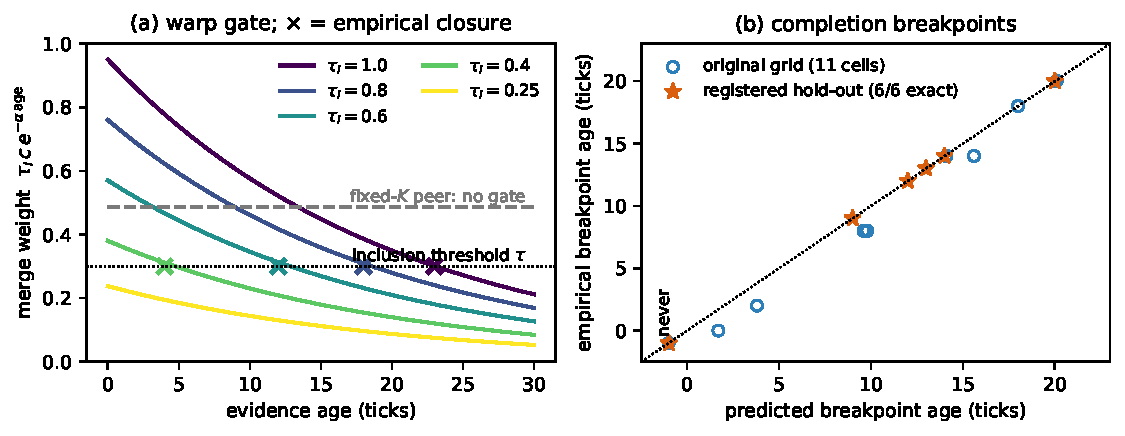
\includegraphics[width=\linewidth]{figures/fig_warp_law}
\caption{The warp distance law. \textbf{(a)} Foreign-evidence merge
weight under trust$\times$staleness decay; $\times$ marks the
empirically measured last age at which the traveller's query still
exposes the target --- each sits on its curve's crossing of the
inclusion threshold $\tau$. Fixed-cadence peer memory has no staleness
term (dashed): its gate never closes; the architectures differ in the
\emph{shape} of the curve. \textbf{(b)} Predicted vs.\ empirical
completion breakpoints in full navigation episodes: original grid
(circles; age sampled in steps of 2, hence points at most one grid
step below the diagonal) and the registered hold-out (stars; age step
1, predictions written to disk before execution, $6/6$ exact,
including the never-cell at $(-1,-1)$ and the cell where the pruning
horizon undercuts the exponential gate).}
\label{fig:law}
\end{figure}

\begin{table}[h]
\centering
\caption{Gate curve: largest evidence age at which the traveller's
query still exposes the target. Fixed-cadence peer memory has no
staleness term: the gate never closes (checked to age 120 at all
trusts) --- the architectures differ in the \emph{shape} of the curve,
not just its level.}
\label{tab:gate}
\small
\begin{tabular}{lcc}
\toprule
trust $\tau_i$ & empirical $\mathrm{age}_{\max}$ & predicted \\
\midrule
1.00 & 23 & 23.05 \\
0.80 & 18 & 18.59 \\
0.60 & 12 & 12.84 \\
0.40 & 4  & 4.73 \\
0.25 & gate closed & 0 (trust-flip) \\
\bottomrule
\end{tabular}
\end{table}

\paragraph{Completion breakpoint.} In full navigation episodes the
feasibility inequality acquires one discrete refinement: the traveller
self-confirms the target once it is within the observation radius, so
the foreign gate only has to survive until tick $t_{\text{gate}} = d -
r_{\text{obs}} - 1$, giving breakpoint $\mathrm{bp} =
\mathrm{age}_{\max} - t_{\text{gate}}$; snapshot pruning executes on
broadcast ticks and adds the bound $10K - t_{\text{bcast}}$. All
constants of the law are unchanged. All 11 CSM cells of the original
grid match within sampling resolution; completion curves are monotone
steps; the trust-flip zeroes $\wstar$ events discretely.

\begin{table}[h]
\centering
\caption{Registered-prediction hold-out: six cells absent from the
original grid, predictions written to disk \emph{before} any episode,
age grid step 1. All six are exact integer matches, including the
never-cell and the cell where the pruning horizon must undercut the
exponential gate.}
\label{tab:holdout}
\small
\begin{tabular}{lccc}
\toprule
Cell & binding bound & predicted & empirical \\
\midrule
$K{=}8$, $\tau_i{=}0.9$, $d{=}9$  & gate    & 14 & \textbf{14} \\
$K{=}8$, $\tau_i{=}0.7$, $d{=}9$  & gate    & 9  & \textbf{9}  \\
$K{=}8$, $\tau_i{=}0.5$, $d{=}15$ & gate    & never & \textbf{never} \\
$K{=}4$, $\tau_i{=}1.0$, $d{=}6$  & gate    & 20 & \textbf{20} \\
$K{=}2$, $\tau_i{=}1.0$, $d{=}12$ & \emph{pruning} & 12 & \textbf{12} \\
$K{=}2$, $\tau_i{=}0.8$, $d{=}8$  & gate    & 13 & \textbf{13} \\
\bottomrule
\end{tabular}
\end{table}

The law is thus predictive out of sample, tick-exactly: the CSM rules
really are the mechanism that forms (and un-forms) intention. It also
reinterprets the companion result that CSM dominates fixed-cadence
peers: trust$\times$staleness is a \emph{warp gate} --- CSM does not
share better, it \emph{refuses to warp on a stale or untrusted song}.

\paragraph{Portability to continuous dynamics.} All three registered
predictions survive on a continuous VMAS substrate through the same
continuous$\to$grid bridge used by the companion's portability test:
(i) the provenance strata stay an order of magnitude apart
($P(\cstar|\wstar)=0.012$ $[0.000,0.042]$ vs.\ $0.562$
$[0.457,0.709]$ at $K{=}1$); (ii) warp share falls monotonically with
cadence ($0.723\to0.366\to0.000$ over $K{=}1/4/16$); (iii) the law
becomes \emph{metric}: with the travel-to-sight time calibrated once
on a fresh-evidence episode, the predicted breakpoints match within
the sampling grid, and all cells beyond the metric warp radius
($v\cdot\mathrm{age}_{\max}$ shorter than the distance) are predicted
\emph{never} and observed \emph{never}. One genuinely continuous
finding: inertia is a physical warp-leak channel --- an agent can
coast into sighting range after the gate closes --- removed by a
no-lock-then-brake controller that restores the grid semantics.

\section{The Warp Drive protocol}
\label{sec:drive}

Warp collision --- locking on foreign evidence for a target someone
else will claim --- is the dominant failure of fast sharing. Warp
Drive adds three primitives, all decentralised:

\begin{enumerate}[leftmargin=20pt,itemsep=2pt,topsep=2pt]
\item \textbf{Optimistic warp lock} --- locks on foreign evidence
  remain allowed immediately (planner unchanged).
\item \textbf{Warp reservation} --- at the owner's next broadcast tick
  the reservation rides on the ordinary snapshot (same cadence $K$, no
  coordinator, no extra channel); receivers suppress reserved targets
  in their queries. Priority: (lock tick, distance at lock, agent id).
\item \textbf{Anti-$\mstar$ rollback} (Time Warp
  semantics~\cite{jefferson1985}) --- an agent holding a lock
  dominated by a foreign reservation retracts it: the planner
  re-queries, the target enters exponential backoff
  ($4\to8\to\cdots\to32$ ticks) with an agent-id tie-break against
  oscillation. The event log stays append-only.
\end{enumerate}

\paragraph{Decentralisation check.} Driving the protocol by direct
per-agent calls --- no runtime, no environment --- produces the same
retraction decisions from each agent's own inbox alone.

\paragraph{Misled-A anchor.} With Warp Drive the pathological lock is
resolved \emph{preventively}: C's reservation arrives before A ever
locks $(3,8)$; A completes on another target. In the sweep, rollback
latency of dominated locks is finite and ${\approx}K$: $1.0/1.5/2.7$
ticks at $K{=}1/2/4$ (baseline: until end of episode).

\begin{figure}[t]
\centering
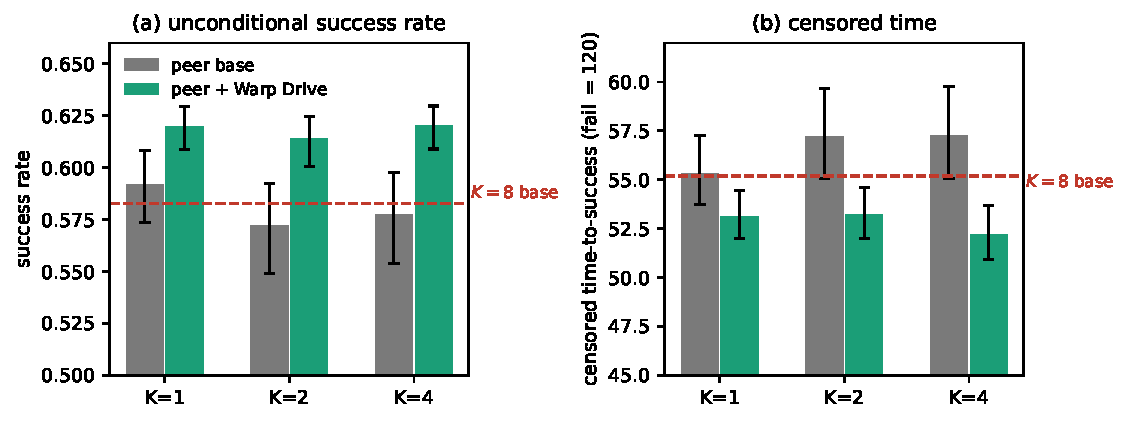
\includegraphics[width=\linewidth]{figures/fig_warp_drive}
\caption{Warp Drive on unconditional metrics (840 episodes; bootstrap
CIs). \textbf{(a)} Success rate rises at every cadence with disjoint
CIs, and every fast-$K$ protocol arm exceeds the $K{=}8$ sweet-spot
baseline (dashed). \textbf{(b)} Censored time-to-success falls
correspondingly. The claim that the protocol removes the main
argument against fast sharing rests on these unconditional
quantities, not on the (denominator-sensitive) conditional rates.}
\label{fig:drive}
\end{figure}

\begin{table}[h]
\centering
\caption{Unconditional results, 840 episodes (scarcity cells
$\times$ random/asymmetric layouts $\times$ 20 seeds). Success rate
rises under Warp Drive at every cadence with disjoint CIs, censored
time falls, and fast sharing with the protocol beats the $K{=}8$
sweet-spot baseline (Figure~\ref{fig:drive}). Lock census shows the
conditional-metric denominator shrinking --- which is why the claim is
stated on unconditional quantities.}
\label{tab:wd}
\small
\begin{tabular}{lccc}
\toprule
Arm & success rate & $t_{\text{cens}}$ (fail $=120$) & lock census \\
\midrule
$K{=}1$ base & 0.592 [0.574, 0.608] & 55.3 [53.7, 57.2] & 0.986 \\
$K{=}1$ +WD  & \textbf{0.620} [0.609, 0.629] & 53.1 [52.0, 54.4] & 0.985 \\
$K{=}2$ base & 0.572 [0.549, 0.592] & 57.2 [55.1, 59.7] & 0.973 \\
$K{=}2$ +WD  & \textbf{0.614} [0.601, 0.624] & \textbf{53.2} [52.0, 54.6] & 0.926 \\
$K{=}4$ base & 0.577 [0.554, 0.598] & 57.3 [55.1, 59.8] & 0.944 \\
$K{=}4$ +WD  & \textbf{0.620} [0.609, 0.630] & \textbf{52.2} [50.9, 53.7] & 0.739 \\
$K{=}8$ base & 0.583 [0.558, 0.604] & 55.2 [52.9, 57.9] & 0.682 \\
\bottomrule
\end{tabular}
\end{table}

On the conditional axis, recovery is measured against the scarcity
ceiling $\min(m,M)/m$ (no protocol conjures extra water): $0.90 / 2.15
/ 6.6$ of the recoverable collapse at $K{=}1/2/4$; values above 1
arise because reservation suppression removes doomed locks from the
$\mstar$ population. Together with Table~\ref{tab:taxi} this closes
the arc: raw warp fails at completion (\S\ref{sec:raw}); with a
coordination contract attached, warp at fast cadence becomes the best
regime. The cadence sweet spot of the companion paper is
reinterpreted: moderate $K$ was never about information freshness ---
it was an implicit rate limiter on warp collisions, and an explicit
contract does the job better.

\section{Cross-session warp on an LLM substrate}
\label{sec:llm}

Finally, the strict warp crosses both an agent boundary and a session
boundary on a language substrate. In session 1, agent A (a local
LLM tag extractor over natural-language observations; Ollama
\method{llama3.1}, deterministic caching, zero API cost) sweeps a
three-room text household and its symbolic memory is dumped to disk.
In session 2, agent B --- a fresh agent in a fresh environment
instance, with the stock directional oracle removed so that long-range
knowledge can only come from memory --- loads A's dump as foreign
provenance and solves ``bring the apple to the table.'' Every lock B
makes on the apple or the table is $\varphi{=}1.0$ strict $\wstar$;
execution is layered (the LLM makes the semantic decisions --- which
remembered place to pursue, when to take/put --- while locomotion to
the locked waypoint is a deterministic motor primitive, matching the
substrate's planner stack).

\begin{table}[h]
\centering
\caption{Cross-session warp over 10 randomised layouts. Completion is
attributed at the environment's affordance radius (take/put act within
Manhattan distance 1, and the witness tags anchors on within-reach
cells).}
\label{tab:llm}
\small
\begin{tabular}{lccc}
\toprule
 & success & mean $t_{\text{succ}}$ & layouts with completed strict $\wstar$ \\
\midrule
warp (A's memory) & \textbf{10/10} & 8.3 & \textbf{10/10} \\
control (empty memory) & 0/10 & --- & --- \\
\bottomrule
\end{tabular}
\end{table}

To our knowledge this is the first documented cross-session,
cross-agent strict semantic warp on an LLM substrate. The $10/10$
vs.\ $0/10$ contrast shows the warp is load-bearing, not decorative.

\paragraph{Scaling to a live collective.} With $N{=}3$ LLM agents
sharing by peer broadcast under scarcity ($M{=}2$ apples, four
layouts, $K\in\{2,8\}$), the full warp phenomenology reproduces on the
language substrate (all predictions registered before the runs):
strict $\wstar$ locks occur; warp share falls with cadence
($0.417$ at $K{=}2$ vs.\ $0.083$ at $K{=}8$ --- the same shape as the
grid $0.554\!\to\!0.105$ and VMAS $0.723\!\to\!0.000$); warp
collisions appear in $7/8$ episodes. A paired comparison against the
no-communication baseline on identical layouts shows raw sharing
\emph{lowering} success from $2/3$ to $1/3$ per episode --- the
collision cost exceeds the information value on the LLM substrate
exactly as in \S\ref{sec:gain}. Attaching the unchanged Warp Drive
protocol to the LLM collective closes the arc on language too: pooled
success rises from $0.333$ to $0.417$ at both cadences with rollback
latencies again ${\approx}K$ ($1$ tick at $K{=}2$, $7$ at $K{=}8$).
The recovery is partial (${\approx}25\%$ of the collapse, vs.\
$90$--$100\%$ on the grid): on a language substrate the collision
pathology is compounded by semantic-level losses (hallucinated anchor
tags, noisy locks) that no reservation can cure --- a measurable
decomposition we leave to future work. The distance law also survives LLM-produced
evidence: with the gate constant $c$ set to the confidence the
extractor actually emitted ($c_{\text{meas}}{=}0.900$), all four
registered breakpoints land within one tick of prediction.

Two interface findings transfer to any LLM-over-symbolic-memory
design: the LLM query former free-generates retrieval tags outside the
memory's vocabulary (requiring an any-of gate), and small local models
are reliable at semantic commitment but not at coordinate arithmetic
or systematic exploration (requiring the layered execution above and
an explicit exploration tier --- without one, discovery never happens
and the warp has nothing to feed on).

\begin{figure}[t]
\centering
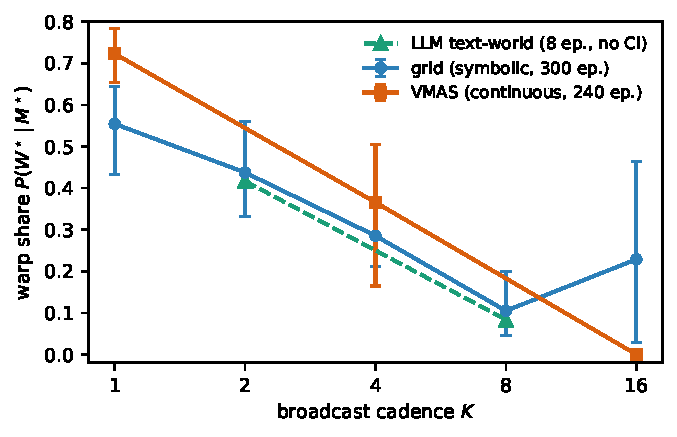
\includegraphics[width=0.62\linewidth]{figures/fig_warp_universality}
\caption{One quantity, three substrates: warp share
$P(\wstar|\mstar)$ vs.\ broadcast cadence $K$ on the symbolic grid,
the continuous VMAS scenario, and the LLM text-world. The curves
nearly coincide --- how much of a collective's materialisation runs
on foreign evidence is set by the sharing cadence, not by the
substrate. (LLM arm: 8 episodes, point estimates only.)}
\label{fig:universality}
\end{figure}

Figure~\ref{fig:universality} overlays the warp-share--cadence curve
across all three substrates: the quantity behaves as a substrate-free
property of the sharing architecture.

\section{Related work}
\label{sec:related}

\paragraph{Shared memory in agent collectives.} Generative
Agents~\cite{park2023generative} and multi-agent LLM frameworks share
memory streams or context but expose no lock interface and no
per-source decomposition of a merged belief, so provenance-conditioned
completion is not measurable there. Vector memories (e.g.\
MemGPT~\cite{packer2023memgpt}) merge by embedding arithmetic;
the merge is not source-decomposable, which blocks both $\varphi$ and
the masked-replay counterfactual.
\paragraph{Emergent communication.} CommNet~\cite{sukhbaatar2016commnet}
and TarMAC~\cite{das2019tarmac} learn continuous channels; the
companion paper shows such channels collapse stage observability. Warp
requires an explicit materialisation event, which these architectures
do not expose.
\paragraph{Stigmergy.} Pheromone-style coordination is an
\emph{anonymous} warp: evidence transfers without provenance. Our
results quantify what anonymity costs (shared-bus warp share is
maximal while its warp completion is minimal) and what
provenance buys (trust gates, reservations, rollback).
\paragraph{Optimistic concurrency.} The rollback primitive is Time
Warp~\cite{jefferson1985} transplanted from parallel simulation to
memory-driven navigation: locks are optimistic computations,
occupancy evidence is a straggler message, anti-$\mstar$ is the
anti-message. To our knowledge this transplant is new.
% TODO: add ALFWorld/TextWorld refs for the LLM substrate; MiniGrid ref.

\section{Limitations and honest negatives}
\label{sec:limits}

(0) All experiments assume a SHARED coordinate frame: place identity
is coordinate proximity with semantics as a tie-breaker inside a
spatial radius; the cross-agent place-correspondence problem is
bracketed, not solved. (A frame-free extension --- fingerprint-based
semantic identity with landmark-consensus frame recovery, failing
closed under perceptual aliasing where the coordinate assumption fails
open --- is implemented and validated separately and is out of scope
here.) (1) Grid worlds, a continuous VMAS scenario, and one small text
world; no photorealistic substrate. (2) The
co-lock-pressure predictor survived only as exploratory
(\S\ref{sec:gain}). (3) The warp-gain sign map is regime-dependent
rather than the clean interior structure the pre-registered
hypothesis expected; deterministic symmetric/asymmetric layouts carry
little seed variance, so the statistical weight rests on random
layouts. (4) The distance-law refinement (self-confirmation horizon,
pruning schedule) was formulated after seeing the original grid ---
mitigated, but not erased, by the registered hold-out. (5) The LLM
demo uses one model family and a deliberately small environment; it is
a demonstration of measurability, not a benchmark. (6) All deviations
from the pre-registered design are listed in
Appendix~\ref{app:deviations}.

\section{Conclusion}

Warp turns ``agents share memory'' from an architecture property into
a measured, causally attributable event with a falsifiable distance
law and a protocol that acts on it. The measurements dissolve the
information-centric reading of collective memory: raw foreign evidence
mostly fails its recipient at completion and pays off as transport,
while a two-line coordination contract --- reserve on lock, roll back
on domination --- makes the fastest sharing regime also the best one.
Provenance, not volume, is the control surface that matters.

\appendix

\section{Deviations from the pre-registered design}
\label{app:deviations}
\begin{enumerate}[leftmargin=20pt,itemsep=2pt,topsep=2pt]
\item Reservation tie-break extended to (lock tick, \emph{distance at
  lock}, agent id): a pure id tie-break hands simultaneous locks to a
  distant agent over the target's near-discoverer.
\item Protocol recovery is measured against the scarcity ceiling
  $\min(m,M)/m$ rather than the $K{=}8$ reference, separating
  structural from coordination collapse; unconditional metrics are
  reported alongside (Table~\ref{tab:wd}).
\item Completion breakpoints use the discrete-time refinement of
  \S\ref{sec:law} (law constants unchanged; hold-out registered).
\item Collision pressure is operationalised as co-lock count rather
  than co-recipients (structurally constant $N{-}2$ under broadcast).
\item LLM demo: layered execution (LLM semantics, deterministic
  locomotion); completion attributed at the affordance radius.
\end{enumerate}

\section{Reproducibility}
\label{app:repro}
All experiments run on CPU in minutes-to-tens-of-minutes; the LLM demo
uses a local Ollama model with deterministic caching.
\begin{verbatim}
PYTHONPATH=. python experiments/warp/exp_warp_anchor.py
PYTHONPATH=. python experiments/warp/exp_warp_gain.py --seeds 20
PYTHONPATH=. python experiments/warp/analyze_warp_chains.py
PYTHONPATH=. python experiments/warp/exp_warp_gain_individual.py
PYTHONPATH=. python experiments/warp/exp_warp_age_law.py
PYTHONPATH=. python experiments/warp/exp_warp_age_law_holdout.py
PYTHONPATH=. python experiments/warp/exp_warp_drive.py --seeds 20
PYTHONPATH=. python experiments/warp/exp_warp_cross_session.py --layouts 10
\end{verbatim}
% TODO: anonymised artifact link for submission.

\section{Full counterfactual sign map}
\label{app:signmap}
% TODO: import the 60-cell sign map from tmp/warp/w1_gain/w1_summary.json
% as a table; include the H-W2 discussion of regime boundaries.

\begin{thebibliography}{9}

\bibitem[Das et~al.(2019)]{das2019tarmac}
A.~Das, T.~Gervet, J.~Romoff, D.~Batra, D.~Parikh, M.~Rabbat, and
J.~Pineau.
\newblock TarMAC: Targeted multi-agent communication.
\newblock In \emph{ICML}, 2019.

\bibitem[Jefferson(1985)]{jefferson1985}
D.~R. Jefferson.
\newblock Virtual time.
\newblock \emph{ACM Transactions on Programming Languages and Systems},
7(3):404--425, 1985.

\bibitem[Packer et~al.(2023)]{packer2023memgpt}
C.~Packer, V.~Fang, S.~G. Patil, K.~Lin, S.~Wooders, and J.~E.
Gonzalez.
\newblock MemGPT: Towards LLMs as operating systems.
\newblock \emph{arXiv:2310.08560}, 2023.

\bibitem[Park et~al.(2023)]{park2023generative}
J.~S. Park, J.~O'Brien, C.~J. Cai, M.~R. Morris, P.~Liang, and M.~S.
Bernstein.
\newblock Generative agents: Interactive simulacra of human behavior.
\newblock In \emph{UIST}, 2023.

\bibitem[Sukhbaatar et~al.(2016)]{sukhbaatar2016commnet}
S.~Sukhbaatar, A.~Szlam, and R.~Fergus.
\newblock Learning multiagent communication with backpropagation.
\newblock In \emph{NeurIPS}, 2016.

\end{thebibliography}

\end{document}
